\documentclass[10pt,conference]{IEEEtran}
\usepackage{graphicx}
\usepackage{amsmath}
\usepackage{cite}
\usepackage{url}
\usepackage{booktabs}
\usepackage{setspace}
\usepackage{xcolor}
\usepackage{caption}
\usepackage{placeins}
\usepackage{enumitem}
\captionsetup{labelsep=period}
\captionsetup[table]{justification=raggedright, singlelinecheck=false}
\setlength{\textfloatsep}{5pt plus 1pt minus 2pt}
\setlength{\floatsep}{5pt plus 1pt minus 2pt}
\setlength{\intextsep}{5pt plus 1pt minus 2pt}

\begin{document}
\setstretch{0.79}

\title{WarpDial: A Case for Reconfigurability and Explainability in Object Storage}

\author{
  \IEEEauthorblockN{Tejus Chandrashekar}
  \IEEEauthorblockA{Independent Researcher\\tchandrashekar@acm.org}
}

\maketitle

\begin{abstract} Object storage offers near-infinite capacity with zero
operational overhead, but its latency can be a concern for HPC and AI
workloads. Managed services hide these low-level
decisions behind an SLA without exposing how the system achieves its
guarantees. Erasure coding is one such decision, providing both storage
efficiency and durability. Giving customers direct control over it is
dangerous because a poor configuration can compromise an object store's
correctness, availability, or durability.

We build WarpDial, a reconfigurability layer on top of
WarpDrive~\cite{warpdrive2026}, an open-source object store. It exposes
static, parametric, and imperative placement policies through one
interface, with an explainability layer that previews and reports each
policy's cost. We validate WarpDial on a nine-node cluster using
DuckDB~\cite{duckdb2019,tpch} and
Lance~\cite{lance2025}. A selective TPC-H query
drops from 723\,ms to 63\,ms ($\sim$11.5$\times$), and Lance row-batch
latency drops from 54\,ms to 19\,ms (up to $\sim$2.9$\times$, less at
higher nprobe), with no change in Recall@10.
\end{abstract}
\FloatBarrier

\section{Introduction}

Object stores typically apply one fixed placement and erasure-coding
policy across an entire pool. Fusion~\cite{fusion2025} shows what
co-designing that policy with the data's own structure can achieve:
aligning erasure-coding stripes with Parquet's column-chunk layout lets
a selective query skip reconstructing a chunk it never requested, at a
reported $\sim$1.2\% storage overhead. We generalize this beyond
Fusion's Parquet-only policy to one interface any operator can
implement for any format, demonstrated here on Parquet analytics and
Lance vector search.

Letting a developer define a policy like Fusion's themselves means
trusting code that decides how an object's bytes are laid out: a wrong
or adversarial policy can silently break the guarantees an object store
exists to provide. We make the following contributions:
\begin{itemize}[leftmargin=*,itemsep=0pt,topsep=0pt,parsep=0pt]
\item \textbf{Interface}: one interface
(\texttt{PlacementPolicy}/\texttt{StripePacker}) that any operator
implements to add a policy, instead of forking the engine.
\item \textbf{Explainability}: a dry-run cost preview before a write,
and a cost report on every PUT response after one, so a caller knows
what a policy costs instead of discovering it blind
(Fig.~\ref{fig:arch}).
\end{itemize}
These policies run today as trusted, compiled-in code, with the same
build-test-deploy cycle as the storage engine itself. For future
workloads, we plan to remove that cycle: a managed service that runs a
tenant's own placement code sandboxed through WebAssembly, with no
build, test, or deploy step of its own, as the caller moves from a
human reviewing each step toward an agent. To our knowledge, no
existing object store exposes this kind of pluggable, cost-reporting
placement interface to developers.

\begin{figure}[t]
  \centering
  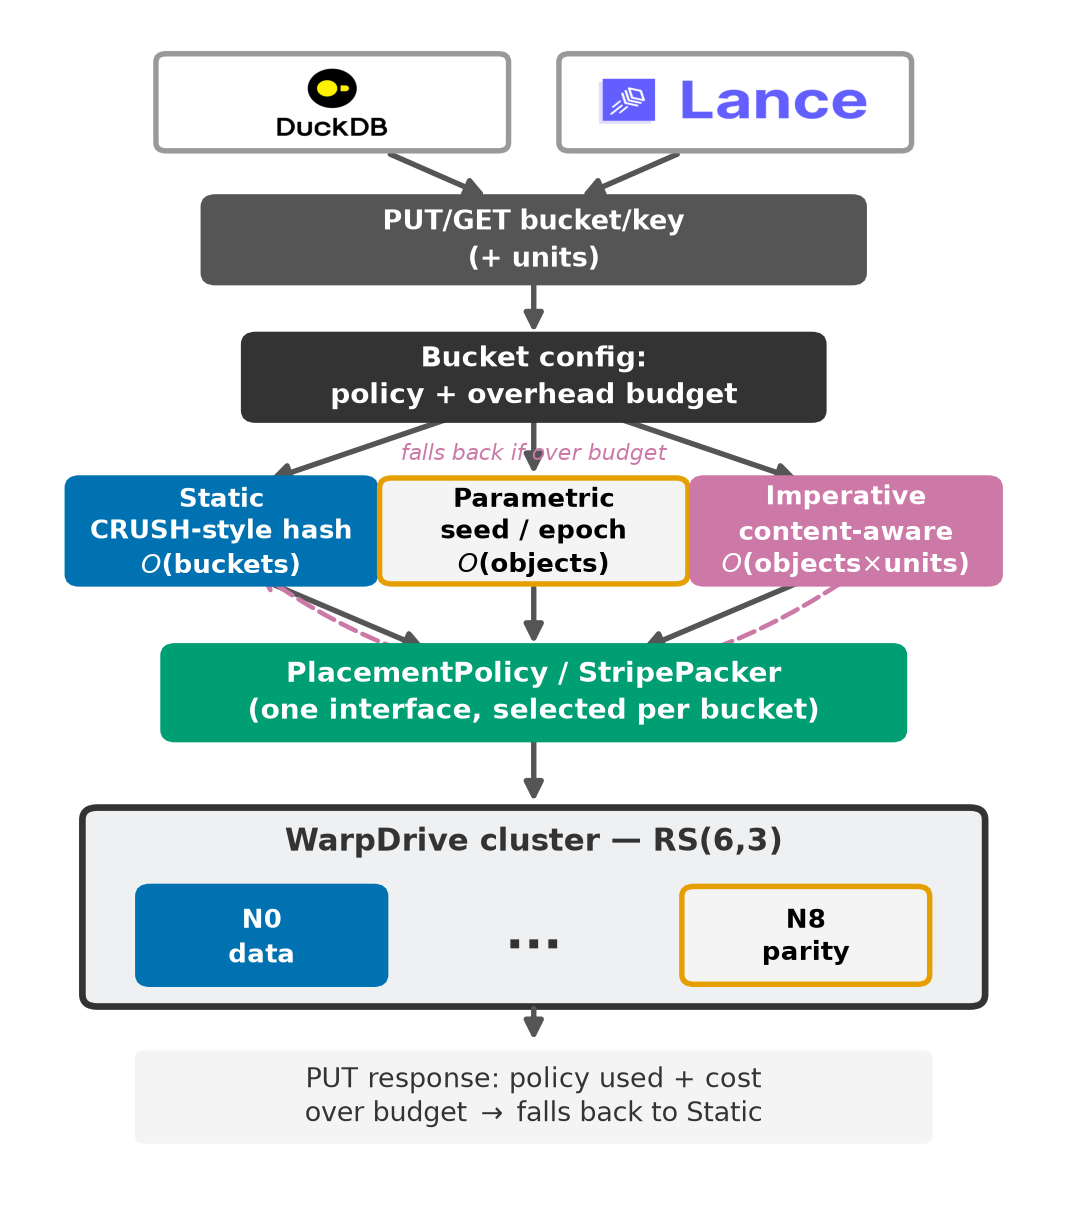
\includegraphics[width=0.66\columnwidth]{plots/architecture.png}
  \caption{WarpDial's architecture: three placement classes behind one
  interface, a per-bucket overhead budget, and a PUT response that
  reports the policy used and its cost.}
  \label{fig:arch}
\end{figure}

\section{Methodology}

Placement classes differ in \emph{who decides location and from what},
and in how much placement state the decision leaves behind. A
\textbf{static} policy derives placement from the object key, bucket
policy, and node set (CRUSH-style hashing): one rule per bucket, no
per-object record, costing $O(\text{buckets})$. A \textbf{parametric}
policy stores a small per-object record (seed, epoch, layout version),
costing $O(\text{objects})$. An \textbf{imperative} policy uses its own
code to decide placement from the object's data itself, workload-aware,
storing one entry per computable unit, costing
$O(\text{objects}\times\text{units per object})$. Fusion's
file-format-aware coding is one imperative policy, hardcoded to
Parquet; we generalize it behind the interface introduced
above, selected per bucket.

We built two concrete imperative policies from an arbitrary
$(\mathit{unit\_id},\mathit{size})$ list and a stripe width $k$: one
groups units by raw size (Fusion's Parquet case or a batch of rows),
the other groups first by IVF cluster ID, then by size, for
vector-index partitions. Both read computable-unit boundaries from a
client-supplied header at PUT time
(\texttt{x-warpd-computable-units: [[offset,len],\ldots]}). Fusion's
own file-format-aware coding discovers these boundaries itself, parsing
a Parquet footer before constructing stripes. We scope our
\texttt{StripePacker} to only the second step; generalizing the first
into this header lets one interface cover Parquet and Lance's
differently structured index without a parser hardcoded to either. A
pluggable parser interface instead, built-in or user-defined per
format, is future work, kept separate from the packer so one packing
algorithm serves many formats and one format serves many algorithms.

A bucket's configuration names its policy and the overhead threshold
described above; exceeding it falls back to static, whole-object
erasure coding. The fallback itself is Fusion's own mechanism, made
per-bucket instead of a single global constant; our own addition is
making its outcome knowable rather than silent. A dry-run endpoint
runs this calculation against
declared units with no body or write, so cost is knowable before
committing, not only after. Letting each bucket pick its own $(k,m)$
stripe width
also loses the uniform failure-domain and free-space accounting a
single pool-wide scheme gives, unmeasured here and left as the natural
next question for running WarpDial across many buckets.

\section{Preliminary Evaluation}

\subsection{Performance}
\label{sec:performance}

A nine-node cluster (one process per node) runs RS(6,3) on one
machine (Apple M3, 8 cores, 16\,GB RAM). We evaluate only the
imperative class, since static and parametric placement
already exist in other object stores, through two variants:
Fusion-style placement for Parquet via DuckDB~\cite{duckdb2019,tpch}
and a new policy for Lance~\cite{lance2025} vector search, each against
a static baseline.

We uploaded the \texttt{dbgen} TPC-H \texttt{lineitem} table and a
Lance IVF\_PQ index over the published SIFT1M-small
corpus~\cite{sift2011}, each once under the static policy and once
under its workload-aware imperative policy, verifying byte-identical
uploads before timing. We ran TPC-H's Q6 (selective) and Q1
(low-selectivity) against the TPC-H upload (Table~\ref{tab:all}). A
separate, larger Lance run (20,000 vectors, 768 dims, 283 partitions)
showed that a query spends most of its time reconstructing the
$\sim$60\,MB row-data fragment, not the small IVF auxiliary file, so we
applied the size-grouped policy to that fragment using 20-row batches.

\begin{table}[t]
\centering
\scriptsize
\setlength{\tabcolsep}{3pt}
\begin{tabular}{@{}lrrr@{}}
\toprule
Workload & stripes touched & bytes reconstructed & overhead \\
\midrule
TPC-H Q6 (sel.) & 1.0/132 & 1.6\,MB/208.5\,MB & 0.21\% \\
TPC-H Q1 (low sel.) & 2.2/132 & 3.5\,MB/208.5\,MB & 0.21\% \\
SIFT1M-small, data & 1.0/84 & 62\,KB/5.1\,MB & 1.18\% \\
SIFT1M-small, aux-idx & 2.6/37 & 23\,KB/311\,KB & \textcolor{red}{412\%} \\
Row-batch, data & 1.0/167 & 368\,KB/61.5\,MB & 0.14\% \\
Row-batch, aux-idx & 2.6/96 & 28\,KB/992\,KB & \textcolor{red}{447\%} \\
\bottomrule
\end{tabular}
\caption{Reconstruction cost per query, RS(6,3): stripes touched, bytes
moved, and overhead, for both the data fragment and IVF aux-index of
each Lance workload.}
\label{tab:all}
\end{table}

\begin{figure}[t]
  \centering
  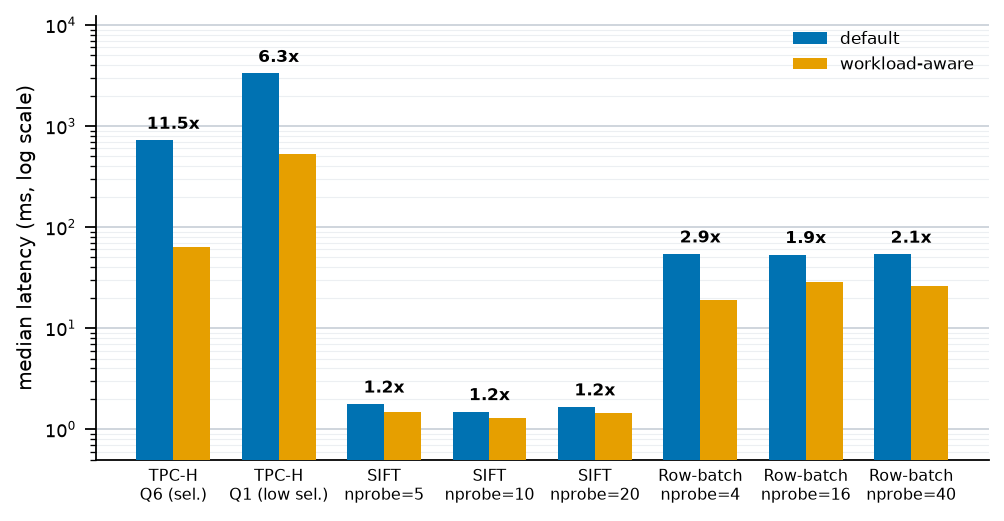
\includegraphics[width=0.56\columnwidth]{plots/all_results_rs63.png}
  \caption{Median latency, RS(6,3), log scale: default
  vs.\ workload-aware placement, across all eight runs.}
  \label{fig:all}
\end{figure}

Table~\ref{tab:all} and Fig.~\ref{fig:all} summarize every result. Q6's
output matched exactly between buckets, as it must: a workload-aware
policy changes how many bytes a query moves, never what it returns, and
the same holds for Recall@10 and the row-batch IDs/vectors. The speedup
tends to track file size: largest on the 208\,MB TPC-H file, smaller on
the 60\,MB row-data fragment, smallest on SIFT1M-small's much smaller
files. The auxiliary index's much higher overhead is expected: a
small object's fixed per-stripe padding and parity cannot be amortized
over many data bytes, which is why every fragment reported here stays
under 1.2\%.

\subsection{Safety and explainability of cost}
\label{sec:safety}

We want every misconfigured or malicious \texttt{StripePacker} rejected
before it writes a shard, not silently accepted. A \texttt{StripePacker}
never sees or supplies an
object's bytes, only which computable unit goes in which bin, how many
bins, and a claimed per-stripe capacity: that is the complete surface it
can lie about.

We test this in two layers. A fast, in-process simulation runs real
\texttt{StripePacker} implementations, each misbehaving one way,
through the same validation a live PUT runs: a
dropped unit, a duplicated unit, a hallucinated unit id, an
out-of-bounds offset, a wrong bin count, and an under-reported capacity
are all rejected before any shard is written. The last is a gap this
testing found and we fixed: capacity was trusted uncritically, letting
an under-report defeat the overhead check and silently truncate real
data past the one existing correctness check. One more case is left
failing on purpose: nothing yet checks a packer's output is
deterministic across calls, unlike the placement-policy interface,
which documents and tests this. Closing that gap, and sandboxing a
packer's \emph{code} rather than only its \emph{output}, is the
WebAssembly direction from the Introduction.

\begin{table}[t]
\centering
\scriptsize
\setlength{\tabcolsep}{3pt}
\begin{tabular}{@{}lllc@{}}
\toprule
Case & Placement & Overhead & Write \\
\midrule
Control (sane) & packed & 0.00\% & ok \\
A (lying header) & plain (fallback) & 500.00\% & ok \\
B (bad packer name) & plain (fallback) & n/a & ok \\
C (capacity-lying packer) & rejected & n/a & failed \\
\bottomrule
\end{tabular}
\caption{Live cases, nine-node RS(6,3), 2\% threshold. A/B retrigger the
camera-ready round's original cases; C is this session's new finding.}
\label{tab:adversarial}
\end{table}

One live case, on the same nine-node RS(6,3) cluster as
Section~\ref{sec:performance}, confirms the fix: a bucket configured
with the same capacity-lying packer is rejected outright
(Table~\ref{tab:adversarial}, Case C), no object left reachable. Cases
A and B retest the original camera-ready round's cases on this cluster.
The dry-run preview's predicted overhead matches the real PUT's
reported overhead exactly for both (0.00\% control, 500.00\% Case A).

\section{Conclusion \& Future Work}

WarpDial gives developers one cost-reporting interface for static,
parametric, and imperative placement policies, the first object store
to do so to our knowledge. On our nine-node cluster it reduces a
selective TPC-H query's latency by $\sim$11.5$\times$ and Lance
row-batch latency by up to $\sim$2.9$\times$, falling to
$\sim$1.9$\times$ at higher nprobe as the plain bucket's own range-GET
path narrows the gap, with query results and Recall@10 unchanged
throughout. The same mechanism keeps placement safe under adversarial
and misconfigured input, detailed in Section~\ref{sec:safety}.

What remains is building the managed-service direction from
Section~\ref{sec:safety}, with the overhead-threshold fallback as a
shared backstop. Other directions include an SLA solver in place of a
single threshold, a multi-VM deployment and comparison against another
erasure-coded store, pool-wide failure-domain/fragmentation effects,
and agent-driven policy configuration.

{\footnotesize\section*{Acknowledgment}
We used AI-agent assistance for language editing and phrasing. We thank all contributors to the WarpDrive source code.
}

{\scriptsize\setstretch{0.85}
\begin{thebibliography}{1}
\setlength{\itemsep}{0pt}
\setlength{\parskip}{0pt}

\bibitem{fusion2025}
J.~Lu \textit{et al.}, ``Fusion: An Analytics Object Store Optimized for
Query Pushdown,'' in \emph{Proc.\ ASPLOS}, 2025.

\bibitem{warpdrive2026}
T.~Chandrashekar, ``WarpDrive: A Composable Storage Substrate for
Disaggregated Data Systems,'' CDMS Workshop, VLDB 2026.

\bibitem{duckdb2019}
M.~Raasveldt and H.~M{\"u}hleisen, ``DuckDB: An Embeddable Analytical
Database,'' in \emph{Proc.\ ACM SIGMOD}, 2019.

\bibitem{tpch}
Transaction Processing Performance Council, ``TPC Benchmark H (Decision
Support),'' Standard Specification.

\bibitem{lance2025}
W.~Pace \textit{et al.}, ``Lance: Efficient Random Access in Columnar
Storage through Adaptive Structural Encodings,'' arXiv:2504.15247, 2025.

\bibitem{sift2011}
H.~J{\'e}gou \textit{et al.}, ``Product Quantization for Nearest Neighbor
Search,'' \emph{IEEE Trans.\ Pattern Anal.\ Mach.\ Intell.}, vol. 33, 2011.

\end{thebibliography}
}

\end{document}
